\documentclass{article}
% Tamaño página
\usepackage[paperheight=27cm,paperwidth=21cm,textwidth=19cm ,textheight=23cm]{geometry}
% Librería lorem ipsum?
\usepackage{lipsum}
\usepackage{fancyhdr}
\usepackage{hyperref}
\usepackage{graphicx}
\graphicspath{{images/}}
\hypersetup{
    colorlinks=true,
    linkcolor=blue,
    filecolor=magenta,      
    urlcolor=cyan,
    pdftitle={Laboratorio 4 - Enlaces WAN - Mariano Campos},
    pdfpagemode=FullScreen,
    }

\title{\bfseries \huge Laboratorio 4 - Enlaces WAN \normalsize{\linebreak\\Redes de computadoras I \\Prof.: Walter Lozano\\Prof.: Alejandro Rodriguez Costello}}
\author{\\\\\\\\\\\\Campos, Mariano Andrés \\ {\small visual.design.90@gmail.com}}
\date{\small 17 de Septiembre 2024}

\begin{document}
    \maketitle
    \newpage

    \section{HDLC}
    El protocolo de control de enlace de datos de alto nivel (High-level Data Link Control), es un protocolo de comunicación que proporciona recuperación de errores en caso de pérdida de paquetes y fallos de secuencias entre otros.\\
    El comando {\bfseries show controllers} ejecutado con privilegios de ejecución, es una herramienta que muestra los canales y si hay conectado o no cables a la interfaz.\\
    El lado del cable R0 es el equipo de comunicación de datos (DCE), y el router R1 es el DTE (Equipo de terminación de Datos).\\ \\
    {\bfseries Diferencias entre DTE y DCE}
    \begin{center}
        \begin{tabular}{| p{9cm} | p{9cm} |}\hline
            {\bfseries DTE} & {\bfseries DCE} \\\hline
            Data Termination Equipement & Data Communicaction Equipement \\\hline
            DTE se ocupa de producir y transferir la información a un DCE. & Convierte señales a un formato apropiado de transmisión del medio y lo inyecta a la red. \\\hline
            Es conectado a una red WAN a través de una red de un DCE. & Una red DCE actúa como intermediario entre dos DTE. \\\hline 
            Ejemplos de DTE: computadoras, impresoras y routers. & Ejemplos de DCE: Modems, adaptadores IDSN (Integrated Services Digital Network).\\\hline
        \end{tabular}
    \end{center}

    \begin{center}
        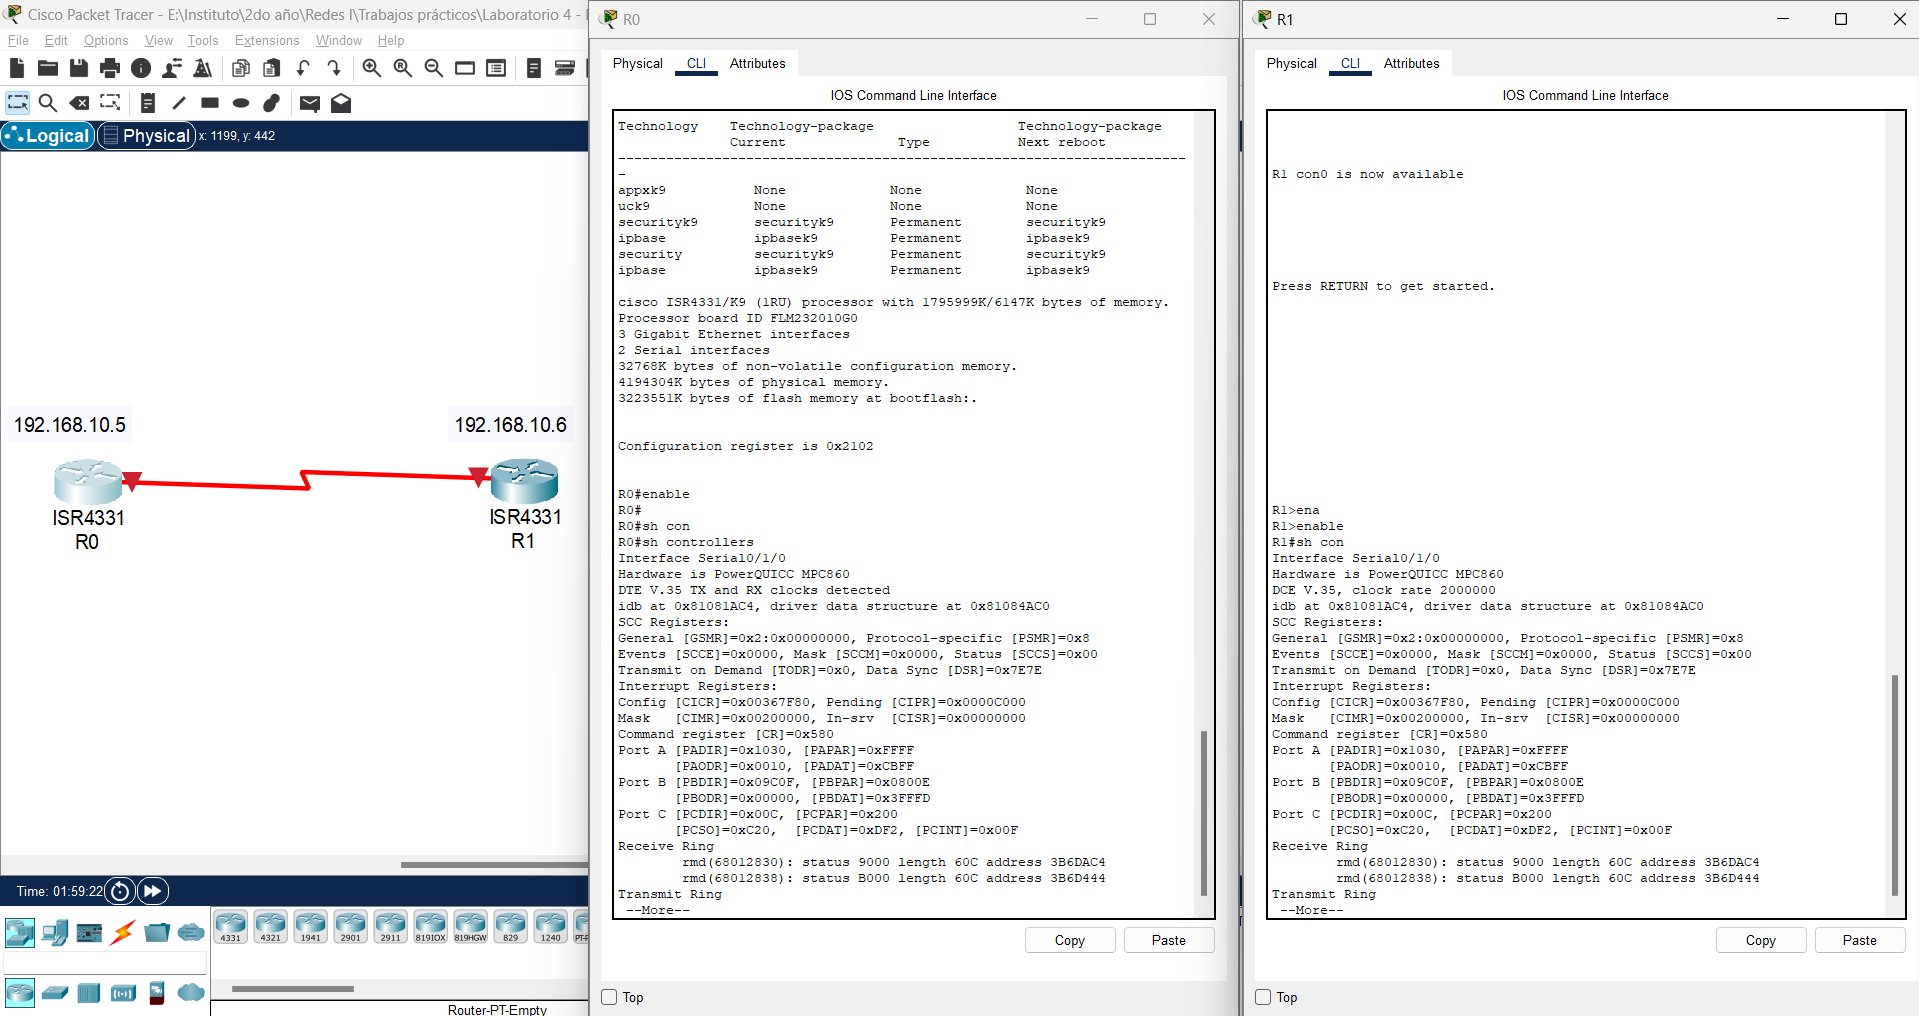
\includegraphics[width=0.875\linewidth]{img_01} 
        \linebreak
        \small {\bfseries Figura 1}: Comando {\bfseries sh con} en ambos routers + update clock rate.
    \end{center}

    Luego de realizar las configuraciones correspondientes, podemos comprobar que la comunicación entre ambos equipos es correcta.\\
    {\bfseries Pasos utilizados para configuración}:
    \begin{enumerate}
        \item R0$>$ ena
        \item R0\# conf t
        \item R0 (config)\# interface serial 0/1/0
        \item R0 (config-if)\# encapsulation hdlc
        \item R0 (config-if)\# no shutdown 
    \end{enumerate}
    Una vez realizads estos pasos en ambos routers podemos comprobar con el comando {\bfseries ping 192.168.10.6} del rounter R0 al router R1, y el comando {\bfseries ping 192.168.10.5} del rounter R1 al router R0.

    \begin{center}
        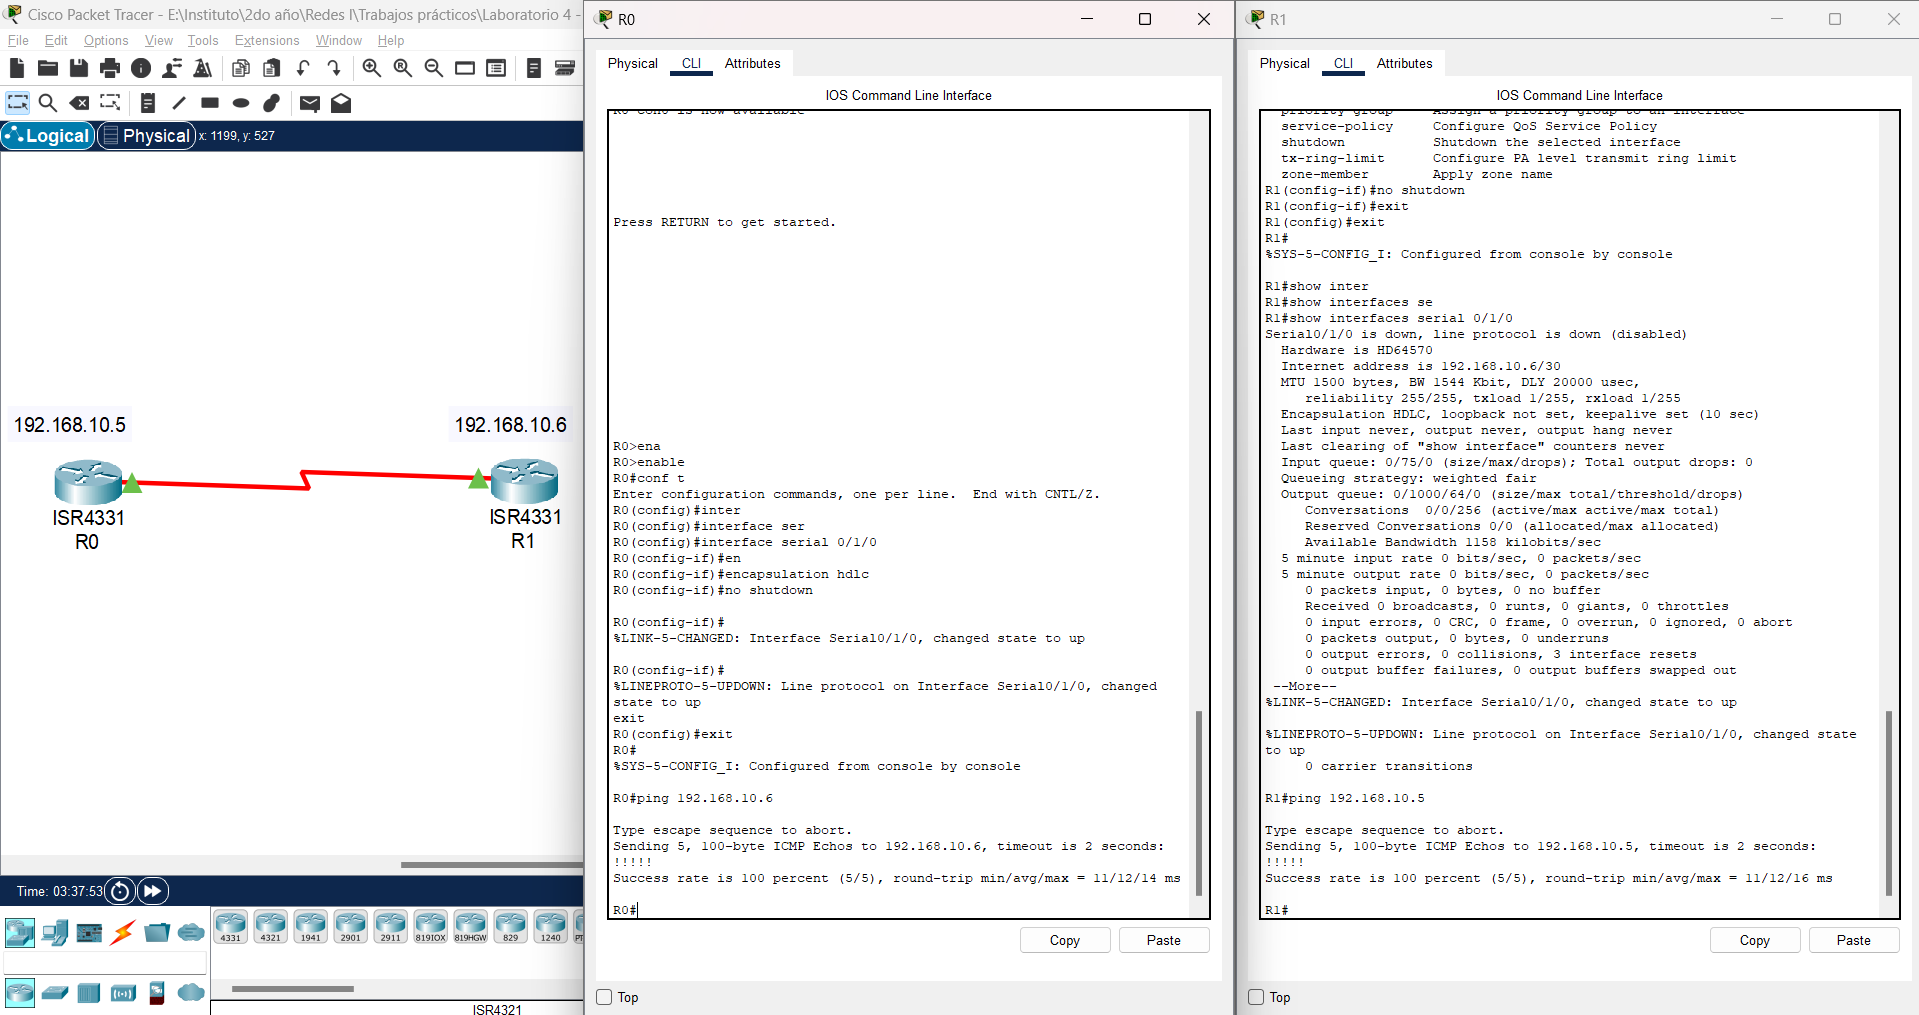
\includegraphics[width=0.875\linewidth]{img_03} 
        \linebreak
        \small {\bfseries Figura 2}: Comprobación de conexión routers R0 y R1.
    \end{center}

    \subsection{Espectos del mecanismo de transmisión}
    \begin{itemize}
        \item Tipos de mensajes SLARP: existen 3 tipos de mensajes definidos para este protocolo:\\
        - address requests (0x00)\\
        - address replies (0x01)\\
        - keep-alive frames (0x02)
        \item Secuencia de los mensajes SLARP: El dispositivo A envía un dispositivo B una paquete con el fin de mantener viva la conexión con un número de secuencia. Posteriormente el dispositivo B envía otro paquete con la solicitud de mantener viva la conexión respondiendo al número de secuencia enviado por A, y un nuevo número de secuencia. Esto se repetirá de manera cíclica cada 10 segundos (por defecto).
        \item Timming de los mensajes SLARP: el tiempo entre los mensajes keep alive es de 10 segundos, y se puede comprobar y/o configurar mediante el comando {\bfseries keepalive (segs.)} en el modo configuración de la interface del terminal (o con el comando show interfaces serial <0-9> en el modo ejecución). Por defecto el protocolo tiene configurado 10 segundos entre paquetes.
        \item Valor de protocol para los mensajes SLARP: SLARP (0x8035)
        \item Valor de protocol para los mensajes unicast: IP (0x0800)
        \item Secuencia de los mensajes unicast: un dispositivo A envía un paquete de solicitud a un dispositivo B el cual enviará un paquete de respuesta al dispositivo A. Un paquete de respuesta por cada paquete de solicitud enviado.
    \end{itemize}

    El secuenciamiento en el protocolo SLARP es importante para asegurar la entrega correcta de paquetes de datos en la red y que no existan errores en la entrega de los mensajes, garantizando llegar en el orden que fueron enviados y así detectar duplicados o paquetes faltantes. El mensaje se distribuye a cada dispositivo de la red.\\
    El secuenciamiento en el protocolo ICMP permite comprobar la conectividad y latencia del anfitrión local con otro equipo de la red. Un ejemplo es el protocolo PING, que permite diagnosticar el estado, velocidad y calidad de una red.\\\\

    {\bfseries ¿Puede identificar el origen y destino de las transmisiones en L2?} \\
    No se puede identificar el origen de las transmisiones debido a que las conexiones son exclusivas. El protocolo HDLC asume que cualquier trama enviada desde un extremo está destinada al otro extremo.

    \section{PPP}
    La autenticación PAP (Password Authentication Protocol) es un subprotocolo cuyo fin es validad a un usuario que accede a ciertos recursos. El ID de usuario y la contraseña viajan en texto plano (no se cifran) por lo que lo hace un protocolo vulnerable a ataques informáticos.\\
    Durante una comunicación PPP en modo PAP, se envía una solicitud de autenticación con el nombre de usuario y contraseña en texto plano y se recibe un paquete ACK con la respuesta afirmativa o negativa sobre la autenticación. Para realizar las configuraciones se realizaron los siguientes pasos (en ambos dispositivos con sus parámetros correspondientes):
    \begin{enumerate}
        \item $R1>$ enable
        \item R1\# conf t
        \item R1 (config)\# interface serial 0/1/0
        \item R1 (config-if)\# authentication pap
        \item R1 (config-if)\# pap sent-username R1 password Cisco1
    \end{enumerate}

    \begin{center}
        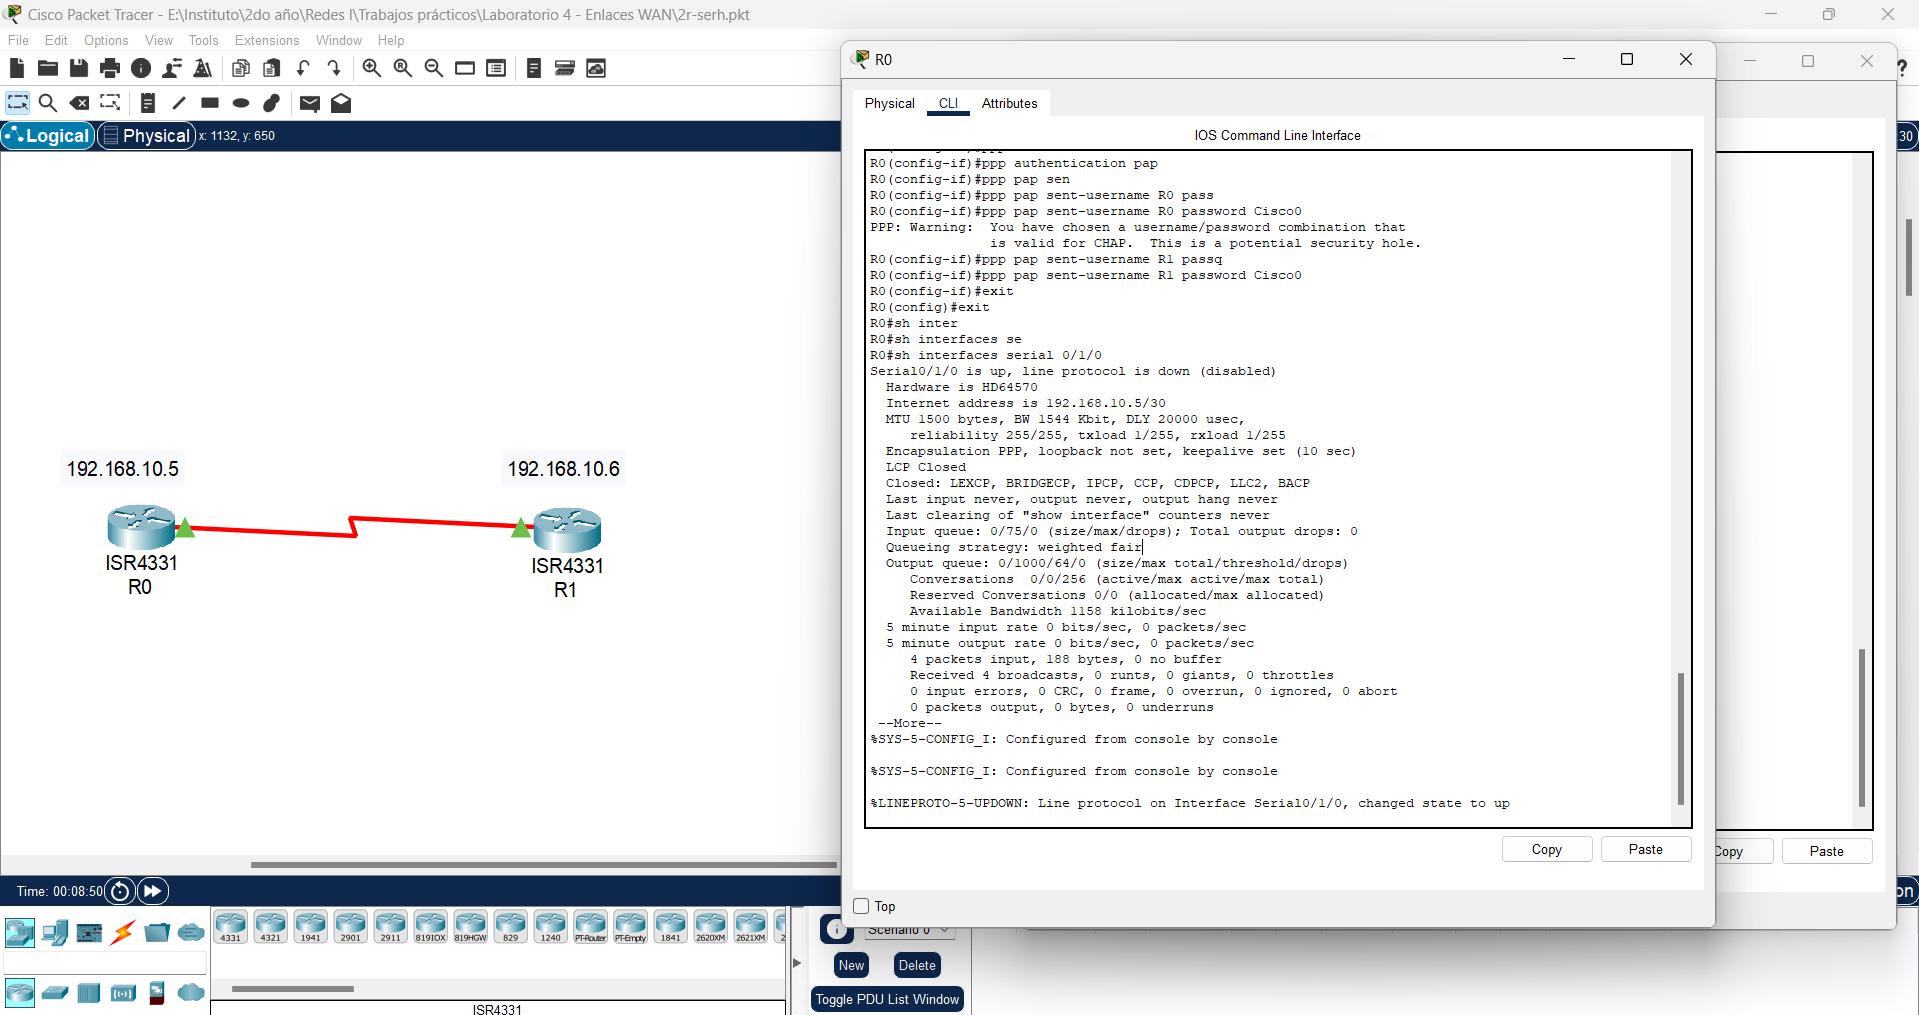
\includegraphics[width=0.875\linewidth]{img_07} 
        \linebreak
        \small {\bfseries Figura 3}: Comprobación de conexión routers R0 y R1 PPP modo PAP.
    \end{center}

    \pagebreak
    \section{Referencias}
        \begin{itemize}
            \item \href{https://github.com/MarianC312/Laboratorio_4_Enlaces_WAN}{Repositorio GitHub}
            \item \href{https://www.cisco.com/c/en/us/td/docs/routers/access/4400/software/configuration/guide/isr4400swcfg.pdf}{Cisco 4000 Series ISRs Software Configuration Guide}
            \item \href{https://ccnadesdecero.es/encapsulacion-hdlc-configuracion-y-resolucion-problemas/}{Encapsulación HLDC - Configuración y resolución de problemas}
            \item \href{https://www.geeksforgeeks.org/difference-between-dte-and-dce/?ref=gcse}{Difference between DTE and DCE}
        \end{itemize}
\end{document}